% !Mode:: "TeX:UTF-8"
\documentclass[12pt,a4paper]{article}

%%%%%%%%------------------------------------------------------------------------
%%%% 日常所用宏包

%% 控制页边距
% 如果是beamer文档类, 则不用geometry
\makeatletter
\@ifclassloaded{beamer}{}{\usepackage[top=2.5cm, bottom=2.5cm, left=2.5cm, right=2.5cm]{geometry}}
\makeatother

%% 控制项目列表
\usepackage{enumerate}

%% 多栏显示
\usepackage{multicol}

%% 算法环境
\usepackage{algorithm}  
\usepackage{algorithmic} 
\usepackage{float} 

%% 网址引用
\usepackage{url}

%% 控制矩阵行距
\renewcommand\arraystretch{1.4}

%% hyperref宏包,生成可定位点击的超链接,并且会生成pdf书签
\makeatletter
\@ifclassloaded{beamer}{
\usepackage{hyperref}
\usepackage{ragged2e} % 对齐
}{
\usepackage[%
    pdfstartview=FitH,%
    CJKbookmarks=true,%
    bookmarks=true,%
    bookmarksnumbered=true,%
    bookmarksopen=true,%
    colorlinks=true,%
    citecolor=blue,%
    linkcolor=blue,%
    anchorcolor=green,%
    urlcolor=blue%
]{hyperref}
}
\makeatother



\makeatletter % 如果是 beamer 不需要下面两个包
\@ifclassloaded{beamer}{
\mode<presentation>
{
} 
}{
%% 控制标题
\usepackage{titlesec}
%% 控制目录
\usepackage{titletoc}
}
\makeatother

%% 控制表格样式
\usepackage{booktabs}

%% 控制字体大小
\usepackage{type1cm}

%% 首行缩进,用\noindent取消某段缩进
\usepackage{indentfirst}

%% 支持彩色文本、底色、文本框等
\usepackage{color,xcolor}

%% AMS LaTeX宏包: http://zzg34b.w3.c361.com/package/maths.htm#amssymb
\usepackage{amsmath,amssymb}
%% 多个图形并排
\usepackage{subfig}
%%%% 基本插图方法
%% 图形宏包
\usepackage{graphicx}
\newcommand{\red}[1]{\textcolor{red}{#1}}
\newcommand{\blue}[1]{\structure{#1}}
\newcommand{\brown}[1]{\textcolor{brown}{#1}}
\newcommand{\green}[1]{\textcolor{green}{#1}}


%%%% 基本插图方法结束

%%%% pgf/tikz绘图宏包设置
\usepackage{pgf,tikz}
\usetikzlibrary{shapes,automata,snakes,backgrounds,arrows}
\usetikzlibrary{mindmap}
%% 可以直接在latex文档中使用graphviz/dot语言,
%% 也可以用dot2tex工具将dot文件转换成tex文件再include进来
%% \usepackage[shell,pgf,outputdir={docgraphs/}]{dot2texi}
%%%% pgf/tikz设置结束


\makeatletter % 如果是 beamer 不需要下面两个包
\@ifclassloaded{beamer}{

}{
%%%% fancyhdr设置页眉页脚
%% 页眉页脚宏包
\usepackage{fancyhdr}
%% 页眉页脚风格
\pagestyle{plain}
}

%% 有时会出现\headheight too small的warning
\setlength{\headheight}{15pt}

%% 清空当前页眉页脚的默认设置
%\fancyhf{}
%%%% fancyhdr设置结束


\makeatletter % 对 beamer 要重新设置
\@ifclassloaded{beamer}{

}{
%%%% 设置listings宏包用来粘贴源代码
%% 方便粘贴源代码,部分代码高亮功能
\usepackage{listings}

%% 设置listings宏包的一些全局样式
%% 参考http://hi.baidu.com/shawpinlee/blog/item/9ec431cbae28e41cbe09e6e4.html
\lstset{
showstringspaces=false,              %% 设定是否显示代码之间的空格符号
numbers=left,                        %% 在左边显示行号
numberstyle=\tiny,                   %% 设定行号字体的大小
basicstyle=\footnotesize,                    %% 设定字体大小\tiny, \small, \Large等等
keywordstyle=\color{blue!70}, commentstyle=\color{red!50!green!50!blue!50},
                                     %% 关键字高亮
frame=shadowbox,                     %% 给代码加框
rulesepcolor=\color{red!20!green!20!blue!20},
escapechar=`,                        %% 中文逃逸字符,用于中英混排
xleftmargin=2em,xrightmargin=2em, aboveskip=1em,
breaklines,                          %% 这条命令可以让LaTeX自动将长的代码行换行排版
extendedchars=false                  %% 这一条命令可以解决代码跨页时,章节标题,页眉等汉字不显示的问题
}}
\makeatother
%%%% listings宏包设置结束


%%%% 附录设置
\makeatletter % 对 beamer 要重新设置
\@ifclassloaded{beamer}{

}{
\usepackage[title,titletoc,header]{appendix}
}
\makeatother
%%%% 附录设置结束


%%%% 日常宏包设置结束
%%%%%%%%------------------------------------------------------------------------


%%%%%%%%------------------------------------------------------------------------
%%%% 英文字体设置结束
%% 这里可以加入自己的英文字体设置
%%%%%%%%------------------------------------------------------------------------

%%%%%%%%------------------------------------------------------------------------
%%%% 设置常用字体字号,与MS Word相对应

%% 一号, 1.4倍行距
\newcommand{\yihao}{\fontsize{26pt}{36pt}\selectfont}
%% 二号, 1.25倍行距
\newcommand{\erhao}{\fontsize{22pt}{28pt}\selectfont}
%% 小二, 单倍行距
\newcommand{\xiaoer}{\fontsize{18pt}{18pt}\selectfont}
%% 三号, 1.5倍行距
\newcommand{\sanhao}{\fontsize{16pt}{24pt}\selectfont}
%% 小三, 1.5倍行距
\newcommand{\xiaosan}{\fontsize{15pt}{22pt}\selectfont}
%% 四号, 1.5倍行距
\newcommand{\sihao}{\fontsize{14pt}{21pt}\selectfont}
%% 半四, 1.5倍行距
\newcommand{\bansi}{\fontsize{13pt}{19.5pt}\selectfont}
%% 小四, 1.5倍行距
\newcommand{\xiaosi}{\fontsize{12pt}{18pt}\selectfont}
%% 大五, 单倍行距
\newcommand{\dawu}{\fontsize{11pt}{11pt}\selectfont}
%% 五号, 单倍行距
\newcommand{\wuhao}{\fontsize{10.5pt}{10.5pt}\selectfont}
%%%%%%%%------------------------------------------------------------------------


%% 设定段间距
\setlength{\parskip}{0.5\baselineskip}

%% 设定行距
\linespread{1}


%% 设定正文字体大小
% \renewcommand{\normalsize}{\sihao}

%制作水印
\RequirePackage{draftcopy}
\draftcopyName{XTUMESH}{100}
\draftcopySetGrey{0.90}
\draftcopyPageTransform{40 rotate}
\draftcopyPageX{350}
\draftcopyPageY{80}

%%%% 个性设置结束
%%%%%%%%------------------------------------------------------------------------


%%%%%%%%------------------------------------------------------------------------
%%%% bibtex设置

%% 设定参考文献显示风格
% 下面是几种常见的样式
% * plain: 按字母的顺序排列,比较次序为作者、年度和标题
% * unsrt: 样式同plain,只是按照引用的先后排序
% * alpha: 用作者名首字母+年份后两位作标号,以字母顺序排序
% * abbrv: 类似plain,将月份全拼改为缩写,更显紧凑
% * apalike: 美国心理学学会期刊样式, 引用样式 [Tailper and Zang, 2006]

\makeatletter
\@ifclassloaded{beamer}{
\bibliographystyle{apalike}
}{
\bibliographystyle{unsrt}
}
\makeatother


%%%% bibtex设置结束
%%%%%%%%------------------------------------------------------------------------

%%%%%%%%------------------------------------------------------------------------
%%%% xeCJK相关宏包

\usepackage{xltxtra,fontspec,xunicode}
\usepackage[slantfont, boldfont]{xeCJK} 
\usepackage{bm}

\setlength{\parindent}{2em}%中文缩进两个汉字位

%% 针对中文进行断行
\XeTeXlinebreaklocale "zh"             

%% 给予TeX断行一定自由度
\XeTeXlinebreakskip = 0pt plus 1pt minus 0.1pt

%%%% xeCJK设置结束                                       
%%%%%%%%------------------------------------------------------------------------

%%%%%%%%------------------------------------------------------------------------
%%%% xeCJK字体设置

%% 设置中文标点样式,支持quanjiao、banjiao、kaiming等多种方式
\punctstyle{kaiming}                                        
                                                     
%% 设置缺省中文字体
%\setCJKmainfont[BoldFont={Adobe Heiti Std}, ItalicFont={Adobe Kaiti Std}]{Adobe Song Std}   
\setCJKmainfont{SimSun}
%% 设置中文无衬线字体
%\setCJKsansfont[BoldFont={Adobe Heiti Std}]{Adobe Kaiti Std}  
%% 设置等宽字体
%\setCJKmonofont{Adobe Heiti Std}                            

%% 英文衬线字体
\setmainfont{DejaVu Serif}                                  
%% 英文等宽字体
\setmonofont{DejaVu Sans Mono}                              
%% 英文无衬线字体
\setsansfont{DejaVu Sans}                                   

%% 定义新字体
\setCJKfamilyfont{song}{Adobe Song Std}                     
\setCJKfamilyfont{kai}{Adobe Kaiti Std}
\setCJKfamilyfont{hei}{Adobe Heiti Std}
\setCJKfamilyfont{fangsong}{Adobe Fangsong Std}
\setCJKfamilyfont{lisu}{LiSu}
\setCJKfamilyfont{youyuan}{YouYuan}

%% 自定义宋体
\newcommand{\song}{\CJKfamily{song}}                       
%% 自定义楷体
\newcommand{\kai}{\CJKfamily{kai}}                         
%% 自定义黑体
\newcommand{\hei}{\CJKfamily{hei}}                         
%% 自定义仿宋体
\newcommand{\fangsong}{\CJKfamily{fangsong}}               
%% 自定义隶书
\newcommand{\lisu}{\CJKfamily{lisu}}                       
%% 自定义幼圆
\newcommand{\youyuan}{\CJKfamily{youyuan}}                 

%%%% xeCJK字体设置结束
%%%%%%%%------------------------------------------------------------------------

%%%%%%%%------------------------------------------------------------------------
%%%% 一些关于中文文档的重定义
\newcommand{\chntoday}{\number\year\,年\,\number\month\,月\,\number\day\,日}
%% 数学公式定理的重定义

%% 中文破折号,据说来自清华模板
\newcommand{\pozhehao}{\kern0.3ex\rule[0.8ex]{2em}{0.1ex}\kern0.3ex}

\newtheorem{example}{例}                                   
\newtheorem{theorem}{定理}[section]                         
\newtheorem{definition}{定义}
\newtheorem{axiom}{公理}
\newtheorem{property}{性质}
\newtheorem{proposition}{命题}
\newtheorem{lemma}{引理}
\newtheorem{corollary}{推论}
\newtheorem{remark}{注解}
\newtheorem{condition}{条件}
\newtheorem{conclusion}{结论}
\newtheorem{assumption}{假设}

\makeatletter %
\@ifclassloaded{beamer}{

}{
%% 章节等名称重定义
\renewcommand{\contentsname}{目录}     
\renewcommand{\indexname}{索引}
\renewcommand{\listfigurename}{插图目录}
\renewcommand{\listtablename}{表格目录}
\renewcommand{\appendixname}{附录}
\renewcommand{\appendixpagename}{附录}
\renewcommand{\appendixtocname}{附录}
%% 设置chapter、section与subsection的格式
\titleformat{\chapter}{\centering\huge}{第\thechapter{}章}{1em}{\textbf}
\titleformat{\section}{\centering\sihao}{\thesection}{1em}{\textbf}
\titleformat{\subsection}{\xiaosi}{\thesubsection}{1em}{\textbf}
\titleformat{\subsubsection}{\xiaosi}{\thesubsubsection}{1em}{\textbf}

\@ifclassloaded{book}{

}{
\renewcommand{\abstractname}{摘要}
}
}
\makeatother

\renewcommand{\figurename}{图}
\renewcommand{\tablename}{表}

\makeatletter
\@ifclassloaded{book}{
\renewcommand{\bibname}{参考文献}
}{
\renewcommand{\refname}{参考文献} 
}
\makeatother

\floatname{algorithm}{算法}
\renewcommand{\algorithmicrequire}{\textbf{输入:}}
\renewcommand{\algorithmicensure}{\textbf{输出:}}

%%%% 中文重定义结束
%%%%%%%%------------------------------------------------------------------------

\numberwithin{equation}{section}
\renewcommand {\thetable} {\thesection{}.\arabic{table}}
\renewcommand {\thefigure} {\thesection{}.\arabic{figure}}
\newcommand{\bbR}{\mathbb{R}}
\newcommand{\bbZ}{\mathbb{Z}}
\newcommand{\bbQ}{\mathbb{Q}}
\newcommand{\bh}{\mathbf{h}}
\newcommand{\bx}{\bm{x}}
\newcommand{\br}{\bm{r}}
%\newcommand{\br'}{\bm{r'}}
\newcommand{\by}{\mathbf{y}}
\newcommand{\bt}{\mathbf{t}}
\newcommand{\bs}{\mathbf{s}}
\newcommand{\bu}{\mathbf{u}}
\newcommand{\bk}{\mathbf{k}}
\newcommand{\bM}{\mathbf{M}}
\newcommand{\bP}{\mathbf{P}}
\newcommand{\bQ}{\mathbf{Q}}
\newcommand{\calS}{\mathcal{S}}
\newcommand{\hF}{\hat{F}}
\newcommand{\bq}{\mathbf{q}}
\newcommand{\hw}{\hat{w}}
\newcommand{\hphi}{\hat{\phi}}
\newcommand{\hxi}{\hat{\xi}}
\newcommand{\hJ}{\hat{J}}

\title{非均相聚合物的平衡理论}
\author{}
\date{\chntoday}
\begin{document}
\maketitle
\section{}
\section{}
\section{}
\section{多链系统的模型}

\subsection{ }

\begin{center}
刘玲
\end{center}

\textbf{4.1.4简化场理论的平均值与算子}

在密度场 $\rho $ 未明显出现的情况下,怎样利用公式$(4.19)-(4.20)$和$(4.30)-(4.31)$的简化场理论计算平均密度和密度相关函数是值得讨论的。\\

我们的出发点是正则系综,用一个包含与微观密度共轭的场$J(\br)$的“源项”来扩展公式$(4.1)$的证明是很方便的。\\
\begin{equation}
Z_{C}[J]=\frac{1}{n! \lambda _{T}^{3n}} \int  \exp \bigg[-\beta U(\br^{n})- \int J(\br) \hat{ \rho }(\br)d\br \bigg]~ d \br^{n}
\end{equation}

$Z_{C}[J]$的对数是一个生成泛函,即$J(\br)$的泛函导数提供了密度的连通(累积量)相关函数。特别是,\\
\begin{equation}
\langle \hat{ \rho } (\br) \rangle = - \frac{\delta \ln Z_{C}[J] }{\delta J(\br)} \bigg |_{J=0}
\end{equation}

其中方程左边的平均值表示粒子在$\br^{n}$位置上的集合平均值。同样,密度相关函数也能得出\\
\begin{equation}
\langle \hat{ \rho } (\br) \hat{ \rho } (\br')\rangle - \langle  \hat{ \rho } (\br) \rangle \langle  \hat{ \rho } (\br') \rangle = \frac{\delta ^{2} \ln Z_{C}[J]}{\delta J(\br) \delta J(\br')} \bigg |_{J=0}
\label{4.44}
\end{equation}

为了计算上述方程右边的导数,追溯$(4.1)$到$(4.19)$的计算步骤到$Z_{C}[J]$的场论表示,这是很有帮助的。显然$u(\br)$必须再次满足必要条件。得到以下场论:\\
\begin{equation}
Z_{C}[J]=Z_{0} \int \exp (-H[w,J]) ~\mathcal{D} w 
\end{equation}
\begin{equation}
H[w ,J]=\frac{1}{2 \beta } \int d\br \int w (\br) u^{-1} (|\br-\br'|) w (\br') - n \ln Q[i w +J] ~d\br'
\end{equation}

其中$J$进入有效哈密顿量仅作为$Q$的一个参数移位,由此得出当$J=0$时,$Z_{C}[0]=Z_{C},H[ w,0]=H[ w ]$。因此,(\ref{4.44})的右侧可以计算\\
\begin{equation}
\langle \hat{ \rho } (\br) \rangle = - n \langle \frac{ \delta \ln Q[i w + J ]}{ \delta J(\br) } \bigg|_{J=0} \rangle = -n \langle \frac{\delta \ln Q[ i w]}{ \delta i w (\br)} \rangle
\label{4.48}
\end{equation}

其中最后两个表达式中的平均值是根据$(4.33)$定义的。这个结果表明我们可以定义一个粒子密度算子\\
\begin{equation}
\tilde{ \rho }(\br;[i w]) \equiv -n \frac{\delta \ln Q[i w]}{\delta i w (\br)} = \frac{\rho _{0}}{Q[i w]} \exp [i w(\br)]
\label{4.49}
\end{equation}
因此\\
\begin{equation}
\langle \hat{ \rho }(\br) \rangle = \langle \tilde{ \rho } (\br;[i w ]) \rangle
\end{equation}

换句话说,$\tilde{ \rho }$是一个算子,其在$ w $场波动的平均值再现了原始粒子模型的平均局部密度$ \langle \hat{ \rho }(\br) \rangle $。注意到(\ref{4.49})中的表达式与$(3.50)$中引入的单个聚合物的段密度算子非常相似。实际上,对于正则系综中的单原子流体,总粒子密度算子$ \tilde{ \rho } $只是单粒子密度算子\\
\begin{equation}
\rho (\br;[i w]) \equiv - \frac{\delta \ln Q[i w]}{\delta i w (\br)}
\end{equation}
乘以粒子数$n$。\\

计算平均局部密度的另一种方法来自类似于推导$(4.39)$的过程。(\ref{4.48})可以写为\\
\begin{equation}
\langle \hat{ \rho } (\br) \rangle = \frac{i}{Z_{C}} \int e^{- (1/2 \beta ) \int d\br \int d\br' w u^{-1} w } \frac{ \delta }{\delta w (\br)} e^{n \ln Q[i w ]} ~\mathcal{D} w
\end{equation}
分部积分可得到\\
\begin{equation}
\begin{aligned}
\langle \hat{ \rho } (\br) \rangle &=\frac{i}{Z_{C}} \bigg[ e^{-A} e^{n \ln Q[i w ]}+\int e^{-A} e^{n \ln Q[i w ]} \frac{1}{2 \beta}(\int wu^{-1}d\br'+\int wu^{-1}d\br) \bigg ]\\&=\frac{i}{\beta}\int u^{-1} d \br' \frac{\int d\br'w \exp(-H[w])}{\int d\br' \exp(-H[w])} \\&= \frac{i}{ \beta } \int u^{-1} (|\br-\br'|) d\br' \langle w (\br') \rangle 
\end{aligned}
\label{4.53}
\end{equation}
因此,粒子密度算子的“替代”表达式可以写为\\
\begin{equation}
\tilde{ \rho }_{a}(\br;[i w ]) \equiv \frac{i}{ \beta } \int  u^{-1}(|\br-\br'|) w (\br')~d\br'
\label{4.54}
\end{equation}
根据$\langle \hat{ \rho }(\br) \rangle = \langle \tilde{ \rho }_{a}(\br;[i \omega ]) \rangle$的性质。注意$\tilde{ \rho } \neq \tilde{ \rho }_{a}$,尽管它们都是计算$(4.19)-(4.20)$中平均局部密度的可接受的算子。\\

“替代方法”对于高阶密度相关函数的评估特别方便。例如,两点函数可以写为\\
\begin{equation}
\begin{aligned}
\langle  \hat{ \rho } (\br) \hat{ \rho } (\br') \rangle &= \frac{1}{Z_{C}[J]} \frac{\delta ^{2}Z_{C}[J]}{\delta J(\br) \delta J(\br')} \bigg|_{J=0} \\&= -\frac{Z_0}{Z_{C}} \int  e^{-(1/2 \beta ) \int d\br \int d\br' w u^{-1} w } \frac{ \delta ^{2} \exp (n \ln Q[i w ])}{\delta w (\br) \delta w (\br')} ~\mathcal{D} w
\end{aligned}
\label{4.55}
\end{equation}
经过两次分部积分得出\\
\begin{equation}
\langle  \hat{ \rho } (\br) \hat{ \rho } (\br') \rangle = - \beta ^{-2} \int d\br_{1}  u^{-1}(|\br-\br_{1}|) u^{-1}(|\br'-\br_{2}|) \langle w(\br_1) w(\br_2)\rangle d\br_{2} + \beta ^{-1} u^{-1} (|\br-\br'|)
\label{4.56}
\end{equation}

从而简化场理论中的密度-密度对相关函数可以由$w$场的对相关函数来计算。\\

上述密度算子和相关函数公式的推导可以很容易地推广到简化理论中的$(4.30)-(4.31)$。给出大正则系综中的粒子密度算子\\
\begin{equation}
\tilde{ \rho }(\br;[i w ]) \equiv -z V \frac{ \delta Q[i w]}{\delta i w (\br)} = z \exp [-i w (\br)]
\end{equation}
所以平均局部粒子密度是\\
\begin{equation}
\langle \tilde{ \rho } (\br) \rangle = \langle \tilde{ \rho }_{G}(\br;[i w ]) \rangle
\end{equation}

右边的平均值是用统计权重$\exp ( -H_{G}[ w])$来表示的,这个表达式与包含$ \rho $场和$ w $场的全理论中的$(4.39)$明显一致。\\

有趣的是,替代粒子密度算子$ \tilde{ \rho }_{a}(\br;[i w])$在正则和大正则系综中都具有相同形式的(\ref{4.54})。因此,用“替代”方程(\ref{4.53})和(\ref{4.56})可以在大正则理论中计算平均局部密度和密度-密度相关函数。据了解,当这些表达式应用于大正则情形时,可以用适当的统计权重$\exp (-H_{G}[ w ])$计算右边的平均值。\\

我们将在整本书中大量参考上述公式。对于只涉及$ w$场的简化场理论,粒子密度算子的各种表达式尤为重要。这些算子公式和相关的统计权重$P[ w ]$汇总在图(\ref{4.1})中。可观测$G[ w]$的集合平均值是根据$(4.33)$应用$P[ w]$定义的\\
\begin{equation}
\langle G[w] \rangle = \frac{\int G[w]P[w]\mathcal{D}w}{\int P[w]\mathcal{D}w}
\end{equation}
\begin{figure}[H]
	\centering   
	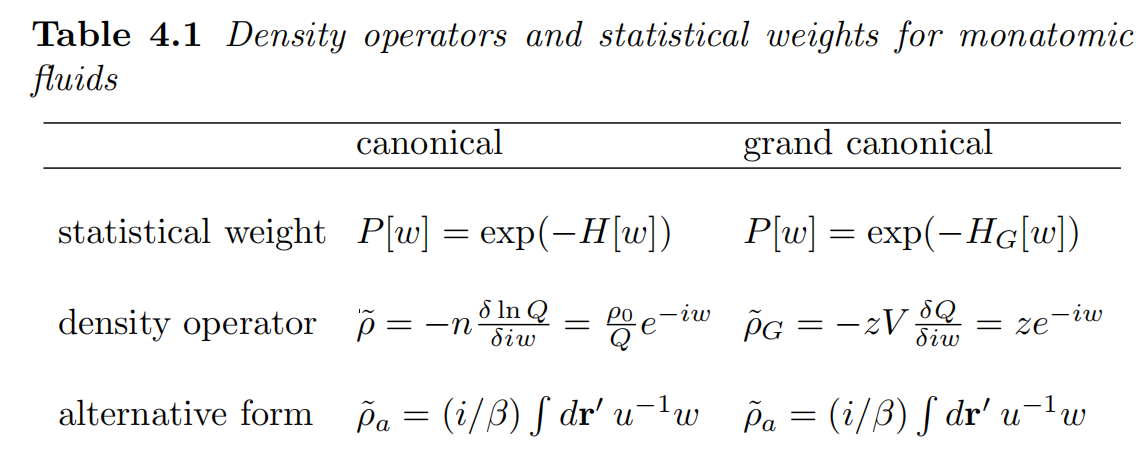
\includegraphics[width=12cm]{./figures/1.png}
	\caption{单原子流体的密度算子和统计权重}
	\label{4.1}
\end{figure}


\subsection{3.2}

\subsection{4.3}

\subsection{4.6液晶聚合物}

液晶聚合物($LCPs$)是含有棒状“液晶”基元的高分子材料,能够在流体-即所谓的液晶状态下产生自发定向秩序。液晶的性质可以有很大不同,这取决于液晶基元的形状和化学细节。向列相、近晶相和胆甾相是最常见的液晶有序情况,但可以找到更复杂的例子,甚至在低分子量液晶中也是如此。德热纳(de Gennes)和普罗斯特(Prost)(1993)的专著对液晶流体的物理学作了很好的介绍。\\

1.\textbf{无序相.}无序相是指空间位置和指向都无序(服从均匀分布)的结构.热致液晶在高温或者溶致液晶在低密度时容易形成无序相;\\

2.\textbf{向列相.}向列相是指空间位置无序、指向有序(所有分子的指向接近平行)的结构;\\

3.\textbf{近晶相.}近晶相是空间和指向都有序的一种微观结构. 与晶体类似,近晶相的空间排列有序,故而称为近晶相,该相是由液晶棒状分子聚集一起,形成一层一层的周期结构,每一层的分子的长轴方向相互平行;\\

4.\textbf{胆甾相.}此类液晶分子呈扁平状,排列成层,层内分子相互平行,分子长轴平行于层平面,不同层的分子长轴方向稍有变化,沿层的法线方向排列成螺旋状结构。\\

当液晶基元被结合到聚合物中时,呈现定向有序相的可能性显著增强。中间基元可以以均匀的方式结合到主链中,也可以连接到侧链上,分别产生主链$LCPs$或侧链$LCPs$。 第二种广义分类是指液晶的顺序通过温度(如所谓的热带)或溶液中聚合物浓度的改变而改变,在这种情况下,液体是热带流体。通过随机共聚合或嵌段/接枝共聚,中间元也可以作为主链或侧链单元并入大分子中。体系结构的复杂性会导致各种现象的发生,其中定向顺序与组合顺序竞争,例如宏相分离或微相分离。\\

由于$LCPs$代表了一组多样的材料,因此在这一范围的专著中不可能提出一套涵盖所有类型的$LCP$系统的全面模型。因此,我们把重点放在一个简单的代表模型主链均聚物系统上,可以显示向列序。模型$G$可以看作是一个热致,主链$LCP$熔体的模型,也可以看作是半柔性聚合物溶致溶液的模型。我们的形式主义类似于以前在文学中出现的描述(Wang和Warner,1986年;Lansac和Maissa,1992年;Gupta和Edwards,1993年;Matsen,1996年;Düuchs和Sullivan,2002年)。\\


\textbf{4.6.1模型G:聚合物分子动力学}

模型$G$是模型$A$的推广,但这里用蠕虫链模型代替了连续高斯链,并加入了聚合物段间的各向异性相互作用。主链向列型聚合物往往是半柔性的,因为中原结合在他们的脊骨。应用蠕虫链模型,默认弯曲阻力沿链是均匀的。对于许多类型的主链$LCPs$来说,这种假设显然是不现实的,但它为理解聚合物的行为提供了一个简单的起点。\\

为了表示各向异性相互作用导致的向列序,将片段位置和取向的微观密度的定义$(3.35)$推广到含有$n$个蠕虫状聚合物的体系中:\\
\begin{equation}
\hat{\rho}(\br,\bu) \equiv \sum_{j=1}^{n} \int _{0}^{L_{c}} \delta(\br-\br_{j}(s)) \delta (\bu-\bu_{j}(s))~ds
\end{equation}

如果我们引用相互作用势的近似,在$\hat{\rho}(\br,\bu)$中,段间非键相互作用对势能的贡献可以描述为二次型:\\
\begin{equation}
U_1=\frac{1}{2} \int d\br \int d\br' \int d\bu \int  \hat{\rho}(\br,\bu) \upsilon_2(\br,\br',\bu,\bu') \hat{\rho}(\br',\bu')~d\bu'
\end{equation}
其中$\upsilon_2$是一个合适的对势函数,假定它在接触时被正则化。我们还了解到,在溶致体系中,$\upsilon_2$为平均力的对势,并取决于纯溶剂的性质。\\

在$LCP$系统的介观描述中,一个典型的进一步逼近是假定在空间上的相互作用是局部的,这相当于$\upsilon_2$的$\delta$函数近似:\\
\begin{equation}
\upsilon_{2}(\br,\br',\bu,\bu') \approx \delta(\br-\br') \upsilon(\bu,\bu')
\end{equation}
其中$\upsilon(\bu,\bu')$是与局部方向相关的相互作用。$\upsilon$的形式不是任意的,它是对称的,并且对于$\bu,\bu'$的符号反转都是不变的。$\upsilon$的常见表达式是昂萨格(Onsager)形式\\
\begin{equation}
\beta \upsilon(\bu,\bu')= u_{1}|\bu\times \bu'|
\end{equation}

它来源于昂萨格的溶致$LCPs$理论和迈尔-索普(Maier-Saupe)形式。\\
\begin{equation}
\beta \upsilon(\bu,\bu')=u_0 - u_{2} P_{2}(\bu \cdot \bu')
\end{equation}

这是热致液晶的迈尔-索普理论的基础。昂萨格形式产生于两个方向为$\bu$和$\bu'$的细长棒之间排除体积的计算,并导致与温度无关(非热)微观长度的预因子$u_{1}>0$。 迈尔-索普形式包含各向同性排除体积项$u_{0}>0$,类似于$(4.62)$,以及一个与$u_2>0$成正比的各向异性四次项。后者乘$P_{2}(\bu,\bu')\equiv (1/2)[3(\bu\cdot \bu')^2-1]$,这是$(2.84)$中定义的二阶勒让德多项式。在原始理论中,假设各向异性系数$u_2$是由范德华尔斯相互作用导出的,因此,在现实中,昂萨格和迈尔-索普形式都是现象学的,因为通过拟合实验数据得到的参数$u_0$、$u_1$和$u_2$的值很少符合这些纯粹熵或纯焓期望。在这两种情况下,稳定向列序的关键是$\upsilon (\bu,\bu')$ 随着两个相邻聚合物段的相互排列而减小。\\

$n$个相互作用的蠕虫链的正则配分函数可以表示为包含上述非键段相互作用的玻尔兹曼因子$\exp (-\beta U_1)$上的$(2.67)$形式的$n$个路径积分的乘积。通过引用模型$A$中的$(4.69)$和$(4.70)$的步骤,可以将这个表达式转换为场论。我们得到以下规范模型$G$场论:\\
\begin{equation}
Z_{C}(n,V,T)=Z_{0} \int \mathcal{D} \rho \int  \exp (-H[\rho,w])~\mathcal{D} w
\end{equation}
有效哈密顿量\\ 
\begin{equation}
H[\rho,w]= -i \int d\br \int d\bu w(\br,\bu) \rho(\br,\bu)-n \ln Q[i w]+\frac{\beta}{2} \int d\br \int d\bu \int  \rho(\br,\bu) \upsilon(\bu,\bu') \rho(\br,\bu')~d\bu'
\end{equation}
其中$Q[i w]$是由$(3.36)$定义的纯虚势$i w(\br,\bu)$中单个蠕虫聚合物链的归一化配分函数。在该模型中,$Z_0$为$n$个非相互作用蠕虫状聚合物链的理想气体的配分函数。\\

在$\upsilon(\bu,\bu')$为正定且具有逆函数的情况下,可以在波动的$\rho(\br,\bu)$场上进行高斯积分,从而在单场$w(\br,\bu)$上实现更简单的场理论。不幸的是,对于昂萨格或迈尔-索普形式,$\upsilon$都不是正定的,这可以很容易地通过球谐展开来验证。因此,模型$G$场理论的简化形式,类似于模型$A$的$(4.71)$和$(4.72)$,对向列相聚合物的适用性有限。\\

在全正则模型$G$场理论中,分段密度$\rho(\br,\bu)$显式出现,因此平均数、段数密度和方向矩可以直接获得。第二个重要的密度算子,只依赖于$w$场,它可以被定义为\\
\begin{equation}
\tilde{\rho}(\br,u;[i w]) \equiv -n \frac{\delta \ln Q[i w]}{\delta i w(\br,\bu)}
\end{equation}

它是$(3.62)$的单链密度算子$\rho(\br,\bu;[i w])$,乘以聚合物数$n$。由此可以从$(3.39)$和$(3.63)$的解中求出这个算子对$w$的特定实现。可以根据$(3.64)-(3.67)$定义其他的压缩段密度算子。\\

另一个$LCPs$中的算子是向列序参数张量$S_{\alpha \beta}(\br;[\rho])$。这个算子虽然不是理论的基础,但可以由\\
\begin{equation}
S_{\alpha \beta}(\br;[\rho]) \equiv \frac{V}{n L_{c}} \int \rho(\br,\bu)(u_{\alpha} u_{\beta}-\frac{1}{3} \delta_{\alpha \beta})~d\bu
\end{equation}

它对$\rho$场波动的期望值为系统中向列序的范围和空间变化提供了一种有用的度量。最后,需要指出的是,在有效哈密顿量$(4.135)$中,用$-n \ln Q$代替$-z VQ$得到了模型$G$场理论的一个巨正则版本。\\

\subsection{4.6液晶聚合物}

液晶聚合物($LCPs$)是含有棒状“液晶”基元的高分子材料,能够在流体-即所谓的液晶状态下产生自发定向秩序。液晶的性质可以有很大不同,这取决于液晶基元的形状和化学细节。向列相、近晶相和胆甾相是最常见的液晶有序情况,但可以找到更复杂的例子,甚至在低分子量液晶中也是如此。德热纳(de Gennes)和普罗斯特(Prost)(1993)的专著对液晶流体的物理学作了很好的介绍。\\

1.\textbf{无序相.}无序相是指空间位置和指向都无序(服从均匀分布)的结构.热致液晶在高温或者溶致液晶在低密度时容易形成无序相;\\

2.\textbf{向列相.}向列相是指空间位置无序、指向有序(所有分子的指向接近平行)的结构;\\

3.\textbf{近晶相.}近晶相是空间和指向都有序的一种微观结构. 与晶体类似,近晶相的空间排列有序,故而称为近晶相,该相是由液晶棒状分子聚集一起,形成一层一层的周期结构,每一层的分子的长轴方向相互平行;\\

4.\textbf{胆甾相.}此类液晶分子呈扁平状,排列成层,层内分子相互平行,分子长轴平行于层平面,不同层的分子长轴方向稍有变化,沿层的法线方向排列成螺旋状结构。\\

当液晶基元被结合到聚合物中时,呈现定向有序相的可能性显著增强。中间基元可以以均匀的方式结合到主链中,也可以连接到侧链上,分别产生主链$LCPs$或侧链$LCPs$。 第二种广义分类是指液晶的顺序通过温度(如所谓的热带)或溶液中聚合物浓度的改变而改变,在这种情况下,液体是热带流体。通过随机共聚合或嵌段/接枝共聚,中间元也可以作为主链或侧链单元并入大分子中。体系结构的复杂性会导致各种现象的发生,其中定向顺序与组合顺序竞争,例如宏相分离或微相分离。\\

由于$LCPs$代表了一组多样的材料,因此在这一范围的专著中不可能提出一套涵盖所有类型的$LCP$系统的全面模型。因此,我们把重点放在一个简单的代表模型主链均聚物系统上,可以显示向列序。模型$G$可以看作是一个热致,主链$LCP$熔体的模型,也可以看作是半柔性聚合物溶致溶液的模型。我们的形式主义类似于以前在文学中出现的描述(Wang和Warner,1986年;Lansac和Maissa,1992年;Gupta和Edwards,1993年;Matsen,1996年;Düuchs和Sullivan,2002年)。\\


\textbf{4.6.1模型G:聚合物分子动力学}

模型$G$是模型$A$的推广,但这里用蠕虫链模型代替了连续高斯链,并加入了聚合物段间的各向异性相互作用。主链向列型聚合物往往是半柔性的,因为中原结合在他们的脊骨。应用蠕虫链模型,默认弯曲阻力沿链是均匀的。对于许多类型的主链$LCPs$来说,这种假设显然是不现实的,但它为理解聚合物的行为提供了一个简单的起点。\\

为了表示各向异性相互作用导致的向列序,将片段位置和取向的微观密度的定义$(3.35)$推广到含有$n$个蠕虫状聚合物的体系中:\\
\begin{equation}
\hat{\rho}(\br,\bu) \equiv \sum_{j=1}^{n} \int _{0}^{L_{c}} \delta(\br-\br_{j}(s)) \delta (\bu-\bu_{j}(s))~ds
\end{equation}

如果我们引用相互作用势的近似,在$\hat{\rho}(\br,\bu)$中,段间非键相互作用对势能的贡献可以描述为二次型:\\
\begin{equation}
U_1=\frac{1}{2} \int d\br \int d\br' \int d\bu \int  \hat{\rho}(\br,\bu) \upsilon_2(\br,\br',\bu,\bu') \hat{\rho}(\br',\bu')~d\bu'
\end{equation}
其中$\upsilon_2$是一个合适的对势函数,假定它在接触时被正则化。我们还了解到,在溶致体系中,$\upsilon_2$为平均力的对势,并取决于纯溶剂的性质。\\

在$LCP$系统的介观描述中,一个典型的进一步逼近是假定在空间上的相互作用是局部的,这相当于$\upsilon_2$的$\delta$函数近似:\\
\begin{equation}
\upsilon_{2}(\br,\br',\bu,\bu') \approx \delta(\br-\br') \upsilon(\bu,\bu')
\end{equation}
其中$\upsilon(\bu,\bu')$是与局部方向相关的相互作用。$\upsilon$的形式不是任意的,它是对称的,并且对于$\bu,\bu'$的符号反转都是不变的。$\upsilon$的常见表达式是昂萨格(Onsager)形式\\
\begin{equation}
\beta \upsilon(\bu,\bu')= u_{1}|\bu\times \bu'|
\end{equation}

它来源于昂萨格的溶致$LCPs$理论和迈尔-索普(Maier-Saupe)形式。\\
\begin{equation}
\beta \upsilon(\bu,\bu')=u_0 - u_{2} P_{2}(\bu \cdot \bu')
\end{equation}

这是热致液晶的迈尔-索普理论的基础。昂萨格形式产生于两个方向为$\bu$和$\bu'$的细长棒之间排除体积的计算,并导致与温度无关(非热)微观长度的预因子$u_{1}>0$。 迈尔-索普形式包含各向同性排除体积项$u_{0}>0$,类似于$(4.62)$,以及一个与$u_2>0$成正比的各向异性四次项。后者乘$P_{2}(\bu,\bu')\equiv (1/2)[3(\bu\cdot \bu')^2-1]$,这是$(2.84)$中定义的二阶勒让德多项式。在原始理论中,假设各向异性系数$u_2$是由范德华尔斯相互作用导出的,因此,在现实中,昂萨格和迈尔-索普形式都是现象学的,因为通过拟合实验数据得到的参数$u_0$、$u_1$和$u_2$的值很少符合这些纯粹熵或纯焓期望。在这两种情况下,稳定向列序的关键是$\upsilon (\bu,\bu')$ 随着两个相邻聚合物段的相互排列而减小。\\

$n$个相互作用的蠕虫链的正则配分函数可以表示为包含上述非键段相互作用的玻尔兹曼因子$\exp (-\beta U_1)$上的$(2.67)$形式的$n$个路径积分的乘积。通过引用模型$A$中的$(4.69)$和$(4.70)$的步骤,可以将这个表达式转换为场论。我们得到以下规范模型$G$场论:\\
\begin{equation}
Z_{C}(n,V,T)=Z_{0} \int \mathcal{D} \rho \int  \exp (-H[\rho,w])~\mathcal{D} w
\end{equation}
有效哈密顿量\\ 
\begin{equation}
H[\rho,w]= -i \int d\br \int d\bu w(\br,\bu) \rho(\br,\bu)-n \ln Q[i w]+\frac{\beta}{2} \int d\br \int d\bu \int  \rho(\br,\bu) \upsilon(\bu,\bu') \rho(\br,\bu')~d\bu'
\end{equation}
其中$Q[i w]$是由$(3.36)$定义的纯虚势$i w(\br,\bu)$中单个蠕虫聚合物链的归一化配分函数。在该模型中,$Z_0$为$n$个非相互作用蠕虫状聚合物链的理想气体的配分函数。\\

在$\upsilon(\bu,\bu')$为正定且具有逆函数的情况下,可以在波动的$\rho(\br,\bu)$场上进行高斯积分,从而在单场$w(\br,\bu)$上实现更简单的场理论。不幸的是,对于昂萨格或迈尔-索普形式,$\upsilon$都不是正定的,这可以很容易地通过球谐展开来验证。因此,模型$G$场理论的简化形式,类似于模型$A$的$(4.71)$和$(4.72)$,对向列相聚合物的适用性有限。\\

在全正则模型$G$场理论中,分段密度$\rho(\br,\bu)$显式出现,因此平均数、段数密度和方向矩可以直接获得。第二个重要的密度算子,只依赖于$w$场,它可以被定义为\\
\begin{equation}
\tilde{\rho}(\br,u;[i w]) \equiv -n \frac{\delta \ln Q[i w]}{\delta i w(\br,\bu)}
\end{equation}

它是$(3.62)$的单链密度算子$\rho(\br,\bu;[i w])$,乘以聚合物数$n$。由此可以从$(3.39)$和$(3.63)$的解中求出这个算子对$w$的特定实现。可以根据$(3.64)-(3.67)$定义其他的压缩段密度算子。\\

另一个$LCPs$中的算子是向列序参数张量$S_{\alpha \beta}(\br;[\rho])$。这个算子虽然不是理论的基础,但可以由\\
\begin{equation}
S_{\alpha \beta}(\br;[\rho]) \equiv \frac{V}{n L_{c}} \int \rho(\br,\bu)(u_{\alpha} u_{\beta}-\frac{1}{3} \delta_{\alpha \beta})~d\bu
\end{equation}

它对$\rho$场波动的期望值为系统中向列序的范围和空间变化提供了一种有用的度量。最后,需要指出的是,在有效哈密顿量$(4.135)$中,用$-n \ln Q$代替$-z VQ$得到了模型$G$场理论的一个巨正则版本。\\


\cite{tam19912d}
\bibliography{../ref}
\end{document}
